\documentclass[11pt,a4paper]{article}
\usepackage[margin=2.4cm]{geometry}
\usepackage{amsmath,amssymb,tikz,parskip,hyperref}
\hypersetup{colorlinks=true,urlcolor=blue}
\title{AI/ML Foundations -- Week 1\\ \large Optimization, Linear Regression and Gradient Descent}
\author{}\date{}
\begin{document}
\maketitle

\section{The big picture}
Most of machine learning follows three steps: choose a \emph{model} with adjustable parameters, choose a \emph{loss} that measures how wrong the model is on data, and \emph{optimize} the parameters to make the loss small. This week covers all three for the simplest useful model: a straight line.

\section{Optimization}
An optimization problem asks for the input that makes a function as small (or large) as possible:
\[ \min_{x \in S} f(x). \]
Here $f$ is the \textbf{objective} and $S$ is the \textbf{feasible set}, the choices we are allowed to make. A point is a \textbf{local minimum} if no nearby feasible point is better, and a \textbf{global minimum} if no feasible point anywhere is better. Maximizing $f$ is the same as minimizing $-f$.

For a differentiable function with no constraints, a minimum must satisfy $\nabla f(x) = 0$. The converse is false in general: maxima and saddle points also have zero gradient.

\section{Linear programming}
In a \textbf{linear program} (LP), both the objective and the constraints are linear. Example:
\[ \max\; 3x + 2y \quad \text{s.t.}\quad x + y \le 5,\;\; x + 3y \le 9,\;\; x \le 4,\;\; x, y \ge 0. \]

\begin{center}
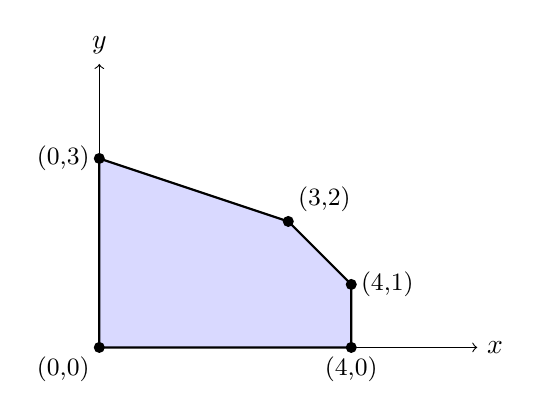
\begin{tikzpicture}[scale=0.8]
\fill[blue!15] (0,0)--(4,0)--(4,1)--(3,2)--(0,3)--cycle;
\draw[->] (0,0)--(6,0) node[right]{$x$};
\draw[->] (0,0)--(0,4.5) node[above]{$y$};
\draw[thick] (0,0)--(4,0)--(4,1)--(3,2)--(0,3)--cycle;
\foreach \p/\l/\a in {(0,0)/{(0,0)}/below left,(4,0)/{(4,0)}/below,(4,1)/{(4,1)}/right,(3,2)/{(3,2)}/above right,(0,3)/{(0,3)}/left}
  {\fill \p circle (2.5pt); \node[\a] at \p {\small \l};}
\end{tikzpicture}
\end{center}

The shaded region is the feasible set. If an LP with such a bounded region has a solution, at least one optimal solution lies at a corner. So we can compare the corners:

\begin{center}
\begin{tabular}{c|ccccc}
corner & $(0,0)$ & $(4,0)$ & $(4,1)$ & $(3,2)$ & $(0,3)$\\ \hline
$3x+2y$ & 0 & 12 & \textbf{14} & 13 & 6
\end{tabular}
\end{center}

The optimum is $14$ at $(4,1)$. Large problems have far too many corners to list. The \textbf{simplex method} starts at one corner and repeatedly moves along an edge to a neighbouring corner that improves the objective, until no improving move remains.

\section{Convexity}
A set is \textbf{convex} if the line segment between any two of its points stays inside it. A function $f$ on a convex set is \textbf{convex} if for all $x, y$ and $t \in [0,1]$,
\[ f(tx + (1-t)y) \le t f(x) + (1-t) f(y), \]
that is, the chord never goes below the graph. A twice-differentiable function is convex exactly when its Hessian is positive semidefinite everywhere (in one variable, $f'' \ge 0$).

\textbf{Why we care:} every local minimum of a convex function is a global minimum. If some point $y$ were better than a local minimum $x$, convexity would make points on the segment just next to $x$ better than $x$ too, which is a contradiction.

\section{Linear regression}
We have data $(x_1, y_1), \dots, (x_n, y_n)$ and want to predict $y$ using $\hat{y} = wx + b$. The \textbf{mean squared error} is
\[ J(w,b) = \frac{1}{n}\sum_{i=1}^{n} (w x_i + b - y_i)^2 . \]
It is convex in $(w,b)$.

\subsection{Closed-form solution}
Set both partial derivatives to zero:
\[ \frac{\partial J}{\partial b} = \frac{2}{n}\sum (w x_i + b - y_i) = 0, \qquad
   \frac{\partial J}{\partial w} = \frac{2}{n}\sum (w x_i + b - y_i)\,x_i = 0. \]
The first gives $b = \bar{y} - w\bar{x}$. Substituting into the second gives
\[ w = \frac{\sum (x_i - \bar{x})(y_i - \bar{y})}{\sum (x_i - \bar{x})^2}, \]
provided the $x_i$ are not all equal.

\textbf{Example.} Points $(1,2), (2,4), (3,5)$: $\bar{x} = 2$, $\bar{y} = 11/3$, so $w = 3/2$ and $b = 2/3$.

\subsection{Matrix form}
Stack the inputs as rows of $X \in \mathbb{R}^{n \times d}$ (with a column of ones for the intercept). Then $J(\theta) = \frac1n \|X\theta - y\|^2$ and $\nabla J = \frac{2}{n} X^\top (X\theta - y)$. Setting it to zero gives the \textbf{normal equations}
\[ X^\top X \theta = X^\top y, \qquad \theta = (X^\top X)^{-1} X^\top y \]
when $X^\top X$ is invertible. In code, solve the system with a least-squares routine instead of computing the inverse.

\textbf{Geometry.} $X\theta$ can only reach vectors in the column space of $X$. The best $X\theta$ is the projection of $y$ onto that space, so the error $y - X\theta$ is perpendicular to every column: $X^\top (y - X\theta) = 0$.

\subsection{Basis functions}
Replace $x$ with features $\phi(x)$, for example $\phi(x) = (1, x, x^2)$. The model $\hat{y} = \theta^\top \phi(x)$ can now draw curves, yet it is still linear in $\theta$, so the same solution applies.

\section{Why squared error? Maximum likelihood}
Assume $y_i = w x_i + b + \varepsilon_i$ with independent noise $\varepsilon_i \sim \mathcal{N}(0, \sigma^2)$. The log-likelihood of the data is
\[ \log L(w,b) = -\frac{n}{2}\log(2\pi\sigma^2) - \frac{1}{2\sigma^2}\sum (y_i - w x_i - b)^2 . \]
Only the last term depends on $w$ and $b$. So \emph{maximizing likelihood is the same as minimizing squared error}.

\section{Gradient descent}
The gradient points in the direction of steepest increase, so we step the opposite way:
\[ \theta_{t+1} = \theta_t - \eta\, \nabla J(\theta_t), \]
where $\eta > 0$ is the \textbf{learning rate}. If $\eta$ is too small, progress is slow; if too large, the steps overshoot and can diverge. For linear regression, gradient descent converges when $\eta < 2/\lambda_{\max}$, where $\lambda_{\max}$ is the largest eigenvalue of the Hessian $\frac{2}{n}X^\top X$.

\textbf{One step by hand.} For the three points above, start at $w = b = 0$. The partial derivatives are $\partial J/\partial w = -50/3$ and $\partial J/\partial b = -22/3$. With $\eta = 0.05$ we get $w \approx 0.833$, $b \approx 0.367$.

\textbf{Feature scaling.} When features have very different scales or are far from zero, the loss surface is a long narrow valley and gradient descent crawls. Standardizing, $z = (x - \bar{x})/s$, makes it much faster.

\textbf{Which to use?} The closed form is exact and needs no learning rate, but solving it costs roughly $O(nd^2 + d^3)$. Each gradient descent step costs only $O(nd)$, and the same method works for models with no closed form.

\section{Practice problems}
\begin{enumerate}
\item Maximize $2x + 3y$ over the feasible region in Section 3.
\item Fit a line to $(0,1), (1,3), (2,4)$ using the closed form.
\item For $f(w) = (w-3)^2$, start at $w = 0$ with $\eta = 0.1$ and take two gradient steps. For which $\eta > 0$ does the method converge?
\item Show that $f(x) = x^2$ is convex using the definition.
\end{enumerate}
\textbf{Answers.} (1) $12$ at $(3,2)$. (2) $w = 3/2$, $b = 7/6$. (3) $w_1 = 0.6$, $w_2 = 1.08$; it converges for $0 < \eta < 1$. (4) The right side minus the left side equals $t(1-t)(x-y)^2 \ge 0$.

\section{Further reading}
\href{https://mml-book.github.io/}{Mathematics for Machine Learning} (Deisenroth, Faisal, Ong): chapters on vector calculus, continuous optimization and linear regression.
\end{document}
